%------------------------------------------------------------------------------
\section{Inverse quantile regression} \label{sec:iqr_method}
%------------------------------------------------------------------------------

%------------------------------------------------------------------------------
\subsection{Main results of IQR}	
%------------------------------------------------------------------------------
Rather than directly optimizing the original GMM objective function in Equation
\ref{eq:gmm_original}, \cite{Chernozhukov2006} propose to do a grid search over
$\alphab$, and each step is a regular quantile regression. They label this process
as "inverse quantile regression" (IQR). The intuition is from the moment
condition in the linear IV quantile regression model in Equation
\ref{eq:moment2}. It implies that the $\tau$-th quantile of $Y -
\Db'\alphab$ conditional on $\Xb$ and $\Zb$ is $\Xb'\betab$:
\begin{align}
Q_{Y - \Db'\alphab_0}(\tau |X, Z) = \Xb' \betab_0 +
\widehat{\Phib}(\tau)'\gammab_0, \qquad \text{with } \gammab_0 = 0 \label{eq:IQR}
\end{align}
where $\widehat{\Phib}(\tau)$ is the transformation of $\Zb$ and $\Xb$. In
practice, $\widehat{\Phib}(\tau)$ is the linear projection of $\Db$ on $\Xb$ and
$\Zb$.

Equation \ref{eq:IQR} means that, based on the true value $\alphab_0$, the
conditional quantile regression of $Y-\Db'\alphab_0$ on $\Xb$ and $\Zb$ will
yield the coefficient on $\widehat{\Phib}(\tau)$ to zero.  Given a sequence of
$\alphab$, denoted as $A = \{\alphab_j\}_{j=1}^J$, we just need to run $J$
regular quantile regression of $ y - \Db'\alphab_j$ on $\Xb$ and
$\widehat{\Phib}(\tau)$.  Denote the estimate for $\gammab_j$ as
$\hat{\gammab}(\alphab_j)$.  Then, the estimator $\hat{\alphab}_{IQR}$ for
$\alphab$ is $\alphab_j$ such that $\hat{\gammab}(\alphab_j)$ is the smallest.
Algorithm \ref{algo:iqr} describes the IQR procedure.

\begin{algorithm}[H]
\caption{Inverse quantile regression} \label{algo:iqr}
\begin{enumerate}
    
\item Define a sequence of $\alphab$'s, denoted by $A = \{\alphab_j\}_{j=1}^J$.

\item Define the quantile level $\tau$.

\item For each variable in $\Db$, compute its linear projection on the space
spanned by $\Xb$ and $\Zb$. Denote the predicted $\Db$ as $\widehat{\Phib}$.

\item For $j$ from $1$ to $J$, make the following loop.

\begin{enumerate}
	\item Run regular $\tau$-th quantile regression of $Y - \Db'\alphab_j$ on
	$\Xb$ and $\widehat{\Phib}$. Denote the estimate for $\betab$ and
	$\gammab$ as $\hat{\betab}(\alphab_j)$ and $\hat{\gammab}(\alphab_j)$,
	respectively.  Also denote the $\hat{\Omegab}(\alphab_j)$ as the estimated
	variance matrix for $\sqrt{N}(\hat{\gammab}(\alphab_j) -
	\gammab(\alphab_j))$.

	\item Compute the norm of $\hat{\gammab}(\alphab_j)$ as $W(\alphab_j) =
	N\hat{\gammab}(\alphab_j)' \hat{\Omegab}(\alphab_j)^{-1}
	\hat{\gammab}(\alphab_j)$
\end{enumerate}

\item The IQR estimate for $\alphab$ is $\hat{\alphab}_{IQR}$ such that
$W(\hat{\alphab}_{IQR})$ is the smallest among $\{W(\alphab_j)\}_{j=1}^J$.
Formally,
\begin{align*}
	\hat{\alphab}_{IQR} = \argmin_{\alphab \in A} W(\alphab)
\end{align*}

\item Given $\hat{\alphab}_{IQR}$, the estimate for $\betab$ is
$\hat{\betab}(\hat{\alphab}_{IQR})$.

\end{enumerate}
\end{algorithm}

\vskip 1cm
To obtain the standard error of the IQR estimator, we have the following
theorem.

\begin{theorem}
\label{thm:iqr_var}
(Theorem 3 in \cite{Chernozhukov2006})
Given some regularity assumptions, for $\epsilon_i(\tau) = Y_i -
\Db_i'\alphab(\tau) - \Xb_i'\betab(\tau)$ and 
$l_i(\tau, \thetab(\tau)) = (\tau - \I (\epsilon_i(\tau) <0))$, 
where $\thetab = (\alphab(\tau), \betab(\tau))$;

\begin{align}
\sqrt{n}(\hat{\thetab}(\cdot) - \thetab(\cdot))
=
- \Jb(\cdot)^{-1} \frac{1}{\sqrt{n}} \sum_{i=1}^n l_i(\cdot,
  \thetab(\cdot))\Psib_i(\cdot) + o_p(1) \implies \bb(\cdot)
\end{align}
where $\bb(\cdot)$ is a mean zero Gaussian process with covariance function
\begin{align*}
\E \bb(\tau) \bb(\tau')' &= \Jb(\tau)^{-1} \Sb(\tau, \tau') [\Jb(\tau')^{-1}]'
\\ \intertext{and}
\Psib_i(\tau) &= (\Phib_i(\tau)', \Xb_i')' \\
\Jb(\tau) &= \E\left[
f_{\epsilon(\tau)}(0|\Xb, \Db, \Zb)\Psib(\tau) [\Db', \Xb']
\right] \\
\Sb(\tau, \tau') &= (\min(\tau, \tau') - \tau \tau') \E \Psib(\tau) \Psib(\tau)'
\end{align*}
where $f_{\epsilon(\tau)}(0| \Xb, \Db, \Zb)$ is the conditional density of
$\epsilon(\tau)$ evaluated at zero.
\end{theorem}

For a discussion on the intuition behind Theorem \ref{thm:iqr_var}, see Section
\ref{sec:discuss_iqrvar}

\begin{remark} \label{iqr:dist} (Remark 3 in \cite{Chernozhukov2006})
A basic implication of Theorem \ref{thm:iqr_var} is that for a given probability
index $\tau$
\begin{align}
	\sqrt{n}(\widehat{\thetab}(\tau) - \thetab(\tau))
	\to N(0, \Jb(\tau)^{-1} \Sb(\tau, \tau) [\Jb(\tau)^{-1}]')
	\label{eq:iqr_var}
\end{align}
Also, for any finite collection of quantile indices ${\tau_j, j \in T}$
\begin{align}
	\{\sqrt{n}(\widehat{\thetab}(\tau) - \thetab(\tau)) \}_{j\in T}
	\to N(0, \{ \Jb(\tau_k)^{-1} \Sb(\tau_k, \tau_l)
	[\Jb(\tau_l)^{-1}]'\}_{k, l \in T})
	\label{eq:iqr_var_tau}
\end{align}
\end{remark}

\begin{remark} \label{iqr:vce} (Remark 4 in \cite{Chernozhukov2006})
The components in the variance matrix in (\ref{eq:iqr_var}) and
(\ref{eq:iqr_var_tau}) can be obtained by its sample counterparts:
\begin{align}
	\widehat{\Sb}(\tau, \tau') = (\min(\tau, \tau') - \tau \tau')
		\frac{1}{n}\sum_{i=1}^n\widehat{\Psib}_i\widehat{\Psib}_i'
\end{align}

The estimator for $\Jb(\tau)$ takes the form
\begin{align}
	\frac{1}{n h_n}\sum_{i}^n K\left(\frac{- \epsilon_i(\tau)}{h_n}\right)
	\widehat{\Psib}_i[\Db_i', \Xb_i']
\end{align}
where $K(\cdot)$ is a Kernel function and $h_n$ is the bandwidth.
\end{remark}
In practice, we can use Kernel as in Stata command {\tt kdensity}. 
For example, the Gaussian Kernel is
$$
K(z) = \frac{1}{\sqrt{2\pi}}e^{-\frac{z^2}{2}}
$$


For the bandwidth, we can use either the Silverman's rule of thumb bandwidth or
the bandwidth used \citeauthor{Koenker2005} (\citeyear{Koenker2005}, Page 81).

The Silverman's rule of thumb bandwidth is 
\begin{align}
  h_{s} = 0.9 
  \min\left(\widehat{\sigma(\epsilon)}, \frac{M}{1.349}\right) 
  n^{-\frac{1}{5}}
\end{align}
where $\widehat{\sigma(\epsilon)}$ is the standard deviation of $\epsilon$ and
$M$ is the interquartile range of $\epsilon$.

The Koenker bandwidth is 
\begin{align}
  h_{k} = 
  \min\left(\widehat{\sigma(\epsilon)}, \frac{M}{1.349}\right) 
  (\Phi^{-1}(\tau + h_1) - \Phi^{-1}(\tau - h_1))
\end{align}
where $h_1$ can be one of the bandwidth in \cite{Hall1988} and
\cite{Bofinger1975}. In particular, 
\begin{align}
	h_{hs} &= n^{-1/3}\Phi^{-1}\left(1 - \frac{\alpha}{2}\right)^{2/3}
	\left[
	\frac{3}{2}\times
	\frac{\phi\left\{\Phi^{-1}(\tau)\right\}^2}
	{2 \Phi^{-1}(\tau)^2 + 1}
\right]^{1/3}
\\
	h_{b} &= n^{-1/5}
	\left[
	\frac{9}{2}\times
	\frac{\phi\left\{\Phi^{-1}(\tau)\right\}^4}
	{\left\{2 \Phi^{-1}(\tau)^2 + 1\right\}^2}
\right]^{1/5}
\end{align}


%------------------------------------------------------------------------------
\subsection{Robust inference approach} \label{sec:iqr_robust}
%------------------------------------------------------------------------------
In the presence of weak instruments the inference is
unreliable. \cite{Chernozhukov2008} proposed an inference approach robust to the
weak instruments. In addition, this approach allows evaluating the quality of
grid specification so that the grid covers the true value of $\alphab$ with a
predefined probability level. 

\begin{prop} \label{prop:robust} (Proposition 1 in \cite{Chernozhukov2008})
When $\alphab =  \alphab(\tau)$,
\begin{align*}
  W_n[\alphab(\tau)] \rightarrow_d \chi^2(dim(\gammab))
\end{align*}
and for the confidence region $CR_p[\alphab(\tau)] = \{\alphab \in A:
W_n(\alphab) < c_p\}$, where $P(\chi^2(dim(\gammab)) < c_p) = p$,
\begin{align}
  P\{\alphab(\tau) \in CR_p[\alphab(\tau)]\} = P\{ W_n[\alphab(\tau)] < c_p\} =
  p
\end{align}
\end{prop}

Intuitively, $W_n(\alphab(\tau))$ is the Wald statistic for testing whether the
coefficients for the instruments are zero ($\hat{\gammab} = 0$). When $\alphab$
equals the true value $\alphab(\tau)$, $W(\cdot)$ is $\chi^2$
distributed with the degree of freedom of dimension of $\gammab$. Thus a valid
confidence interval for $\alphab$ can be constructed by the inversion of the
Wald statistic. That is 
$$
CR_p[\alphab(\tau)] = \{\alphab \in A: W_n(\alphab) < c_p\}
\text{ cover the true value of $\alphab$ with probability approaching
$p$}
$$

The confidence region is a byproduct of the inverse quantile regression.
Algorithm \ref{algo:iqr_robust} is an extension of algorithm \ref{algo:iqr} so
that the robust confidence region is computed. Following
\cite{Chernozhukov2008}, the robust confidence interval $CR_p$ is also called 
dual confidence interval, abbreviated as dual CI.

\begin{algorithm}[H]
\caption{Inverse quantile regression with robust inference}
\label{algo:iqr_robust}

\begin{enumerate}
    % import the iqr algorithm
  
\item Define a sequence of $\alphab$'s, denoted by $A = \{\alphab_j\}_{j=1}^J$.

\item Define the quantile level $\tau$.

\item For each variable in $\Db$, compute its linear projection on the space
spanned by $\Xb$ and $\Zb$. Denote the predicted $\Db$ as $\widehat{\Phib}$.

\item For $j$ from $1$ to $J$, make the following loop.

\begin{enumerate}
	\item Run regular $\tau$-th quantile regression of $Y - \Db'\alphab_j$ on
	$\Xb$ and $\widehat{\Phib}$. Denote the estimate for $\betab$ and
	$\gammab$ as $\hat{\betab}(\alphab_j)$ and $\hat{\gammab}(\alphab_j)$,
	respectively.  Also denote the $\hat{\Omegab}(\alphab_j)$ as the estimated
	variance matrix for $\sqrt{N}(\hat{\gammab}(\alphab_j) -
	\gammab(\alphab_j))$.

	\item Compute the norm of $\hat{\gammab}(\alphab_j)$ as $W(\alphab_j) =
	N\hat{\gammab}(\alphab_j)' \hat{\Omegab}(\alphab_j)^{-1}
	\hat{\gammab}(\alphab_j)$
\end{enumerate}

\item The IQR estimate for $\alphab$ is $\hat{\alphab}_{IQR}$ such that
$W(\hat{\alphab}_{IQR})$ is the smallest among $\{W(\alphab_j)\}_{j=1}^J$.
Formally,
\begin{align*}
	\hat{\alphab}_{IQR} = \argmin_{\alphab \in A} W(\alphab)
\end{align*}

\item Given $\hat{\alphab}_{IQR}$, the estimate for $\betab$ is
$\hat{\betab}(\hat{\alphab}_{IQR})$.


  \item The dual confidence region for $\alphab(\tau)$, $CR_p$, can be computed
    as $CR_p[\alphab(\tau)]  = \{ \alphab_j : W_n(\alphab_j) < c_p \}$, where
    $P(\chi^2(dim(\gammab)) < c_p) = p$. By default, $p = 0.95$.  The upper and
    lower bound of $CR_p(\alphab(\tau)$ may be used as endpoints of confidence
    interval for $\alphab(\tau)$

  \item If $CR_p$ is empty, $\Ab$ is not a valid grid specification because the
    true value of $\alphab(\tau)$ is not covered by $\Ab$ with a big probability.

\end{enumerate}

\end{algorithm}

%------------------------------------------------------------------------------
\subsection{Initial grid}
%------------------------------------------------------------------------------
The initial grid points are computed using the two-stage-quantile regression,
extending the two-stage-median regression in \cite{Amemiya1982}.
The quality of the initial grid can be evaluated using the dual CI. The
implementation requires that the initial grid interval be wider than the
dual CI. Otherwise, {\tt ivqregress iqr} will error out.

A simulation is run to evaluate the effectiveness of the dual CI. In particular,
in a repeated sampling setting, we compute the coverage rate of the dual CI.  In
each repetition, we compute the coverage indicator, which is either 1 if the
true value is within the dual CI or 0 otherwise. The coverage is the average of
the indicator variable over $1000$ repetitions. The sample size is set to
$1000$.  Given the default 95\% level, the coverage rate of the dual CI should
be close to $0.95$. Figure \ref{fig:dualci} plots the coverage rate of dual CI
at different quantile estimates. As expected, the dual CI can cover the
true value with a probability close to $95\%$.

\begin{figure}[H]
\caption{dual 95\% CI coverage rate}
\label{fig:dualci}
\centering
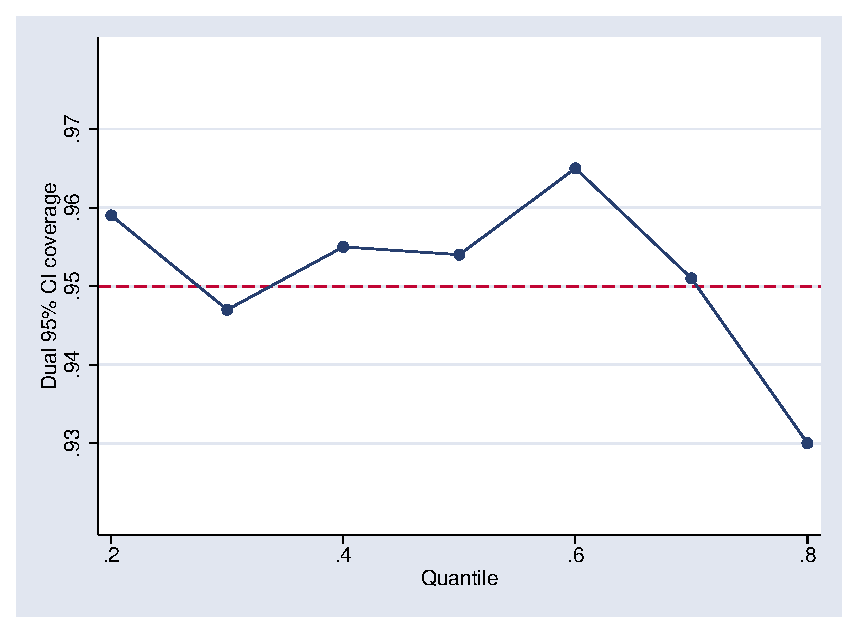
\includegraphics[scale=0.8]{eps/dualci}
\end{figure}

The two-stage-quantile regression is computed in the following steps.

\begin{enumerate}
  \item Compute $\hat{\Phib}(\tau)$, which is the linear projection of $\Db$ on
  $\Xb$ and $\Zb$.
  \item Run a quantile regression of $Y$ on $\Xb$ and $\hat{\Phib}(\tau)$.
  Denote $\tilde{\alphab}$ as the point estimates for the coefficient on
  $\hat{\Phib}(\tau)$ and $\tilde{s}$ as its standard errors.  $\tilde{s}$ is
  computed by assuming the error term is normally distributed.
  \item Compute the lower and upper bound of the grid. The lower bound is
    $lb = \tilde{\alphab} - 4\tilde{s}$, and the upper bound is 
    $ub = \tilde{\alphab} + 4\tilde{s}$.
  \item By default, the grid points are 30 equally spaced points between $lb$
  and $ub$. We can also specify the number of grid points in option {\tt
  ngrid()}.
\end{enumerate}

We show one example to illustrate the connection between the dual CI
and the grid.  To fix the idea, we fit an IVQR model using the simulated data.
First, we fit the inverse quantile regression of $y$ on the endogenous $d1$ and
exogenous $x1$ and $x2$, and use $z1$ and $z2$ as instruments.

\begin{stlog}
. ivqregress iqr y x1 x2 (d1 = z1 z2),  quantile(40) noadaptive
{\smallskip}
Initial grid
    quantile = 0.40: .........10.........20.........30
{\smallskip}
IV .4 quantile regression                              Number of obs =   1,000
Estimator: Inverse quantile regression                 Wald chi2(3)  = 3534.04
                                                       Prob > chi2   =  0.0000
{\smallskip}
\HLI{13}{\TOPT}\HLI{64}
             {\VBAR}               Robust
           y {\VBAR} Coefficient  std. err.      z    P>|z|     [95\% conf. interval]
\HLI{13}{\PLUS}\HLI{64}
          d1 {\VBAR}    .459274   .0502662     9.14   0.000      .360754    .5577939
          x1 {\VBAR}   1.393901   .0334069    41.72   0.000     1.328425    1.459377
          x2 {\VBAR}   1.427885   .0321419    44.42   0.000     1.364888    1.490882
       _cons {\VBAR}  -.3458003   .0411389    -8.41   0.000     -.426431   -.2651695
\HLI{13}{\BOTT}\HLI{64}
Endogenous: d1
 Exogenous: x1 x2 z1 z2
{\smallskip}

\end{stlog}

By default, the initial grid is computed by the two-stage-quantile regression.
We now plot the Wald statistic for each point in the grid. 

\begin{stlog}
\input{logs/log_wald2.log.tex}
\end{stlog}

\begin{figure}[H]
\caption{Wald statistic plot}
\label{fig:dualci}
\centering
\includegraphics[scale=0.3]{eps/waldplot}
\end{figure}

In the above graph, the Wald statistics are plotted for each point in the grid.
The critical value of the Wald statistic is shown as a red horizontal dash line.
The dual CI is the grid points such that the corresponding Wald statistic is
smaller than the critical value, shown in the red shaded area. 

From the above graph, we can visually inspect two features regarding the
estimation. First, we see that the point estimate results in the minimum of the
Wald statistic. Second, we see that the point estimate is within the $95\%$ dual
CI and the initial grid interval is wider than the dual CI. Thus, we are $95\%$
or more confident that the initial grid interval contains the true value of the
parameter.

To see the numerical values of the dual CI, we use {\tt estat dualci}.

\begin{stlog}
. estat dualci
{\smallskip}
Dual confidence interval                                 Number of obs = 1,000
\HLI{13}{\TOPT}\HLI{64}
             {\VBAR}               Robust                               Dual
           y {\VBAR} Coefficient  std. err.      z    P>|z|     [95\% conf. interval]
\HLI{13}{\PLUS}\HLI{64}
          d1 {\VBAR}    .459274   .0502662     9.14   0.000     .3835663    .5728356
\HLI{13}{\BOTT}\HLI{64}

\end{stlog}

%------------------------------------------------------------------------------
\subsection{Adaptive grid search}
%------------------------------------------------------------------------------
Sometimes, a point estimate is found in a flat region, which implies some
degree of weak identification of the parameter. The weak identification can be
caused by the weak identified model or the coarse grid points. The
adaptive grid search can help alleviate the weak identification issue caused by
the coarse grid points. However, the adaptive grid search can not help if the
model is intrinsically weakly identified.

The adaptive grid search is conducted in the following steps.

\begin{enumerate}
  \item Based on the initial grid points, compute the inverse quantile
    regression and the dual CI. 
  \item Construct a new grid using the dual CI, that is, construct several
    equally spaced points between the lower and upper bound in the dual CI.
  \item Compute the inverse quantile regression using the grid in 
    step 2.
\end{enumerate}

Here is one example. First, we fit a IVQR model using the original grid and
plot the Wald statistics.

\begin{stlog}
\input{logs/log_wald4.log.tex}
\end{stlog}

\begin{figure}[H]
\caption{Wald statistic plot}
\label{fig:dualci}
\centering
\includegraphics[scale=0.3]{eps/waldplot_asset}
\end{figure}

The Wald plot shows that the minimum is found in a flat region. Now, we refit
the IVQR model but using the adaptive grid search.

\begin{stlog}
. use assets2, clear
(Excerpt from Chernozhukov and Hanson (2004) Rev. of Economics and Statistics)
{\smallskip}
. 
. ivqregress iqr assets (i.p401k = i.e401k) income age familysize ///
>         i.married i.ira i.pension i.ownhome educ, quantile(50) 
{\smallskip}
Initial grid
    quantile = 0.50: .........10.........20.........30
{\smallskip}
Adaptive grid
    quantile = 0.50: .........10.........20.........30
{\smallskip}
IV median regression                                   Number of obs =   9,913
Estimator: Inverse quantile regression                 Wald chi2(9)  = 1289.75
                                                       Prob > chi2   =  0.0000
{\smallskip}
\HLI{13}{\TOPT}\HLI{64}
             {\VBAR}               Robust
      assets {\VBAR} Coefficient  std. err.      z    P>|z|     [95\% conf. interval]
\HLI{13}{\PLUS}\HLI{64}
     1.p401k {\VBAR}   5313.397   573.2818     9.27   0.000     4189.786    6437.009
      income {\VBAR}   .1577512   .0124889    12.63   0.000     .1332735    .1822289
         age {\VBAR}   99.96526   8.561923    11.68   0.000      83.1842    116.7463
  familysize {\VBAR}  -197.8251   54.36773    -3.64   0.000    -304.3838   -91.26627
             {\VBAR}
     married {\VBAR}
    Married  {\VBAR}  -1359.124   227.3366    -5.98   0.000    -1804.696   -913.5528
             {\VBAR}
         ira {\VBAR}
        Yes  {\VBAR}   22629.61   1022.706    22.13   0.000     20625.15    24634.08
             {\VBAR}
     pension {\VBAR}
Receives ..  {\VBAR}  -693.8347   210.6176    -3.29   0.001    -1106.638   -281.0317
             {\VBAR}
     ownhome {\VBAR}
        Yes  {\VBAR}  -30.29657   154.7265    -0.20   0.845     -333.555    272.9618
        educ {\VBAR}  -96.43983   32.09465    -3.00   0.003    -159.3442   -33.53547
       _cons {\VBAR}  -4998.673   570.1315    -8.77   0.000     -6116.11   -3881.236
\HLI{13}{\BOTT}\HLI{64}
Endogenous: 0b.p401k 1.p401k
 Exogenous: income age familysize 0b.married 1.married 0b.ira 1.ira
            0b.pension 1.pension 0b.ownhome 1.ownhome educ 0b.e401k 1.e401k
{\smallskip}
. 
. estat waldplot, name(b)

\end{stlog}

\begin{figure}[H]
\caption{Wald statistic plot}
\label{fig:dualci}
\centering
\includegraphics[scale=0.3]{eps/waldplot_asset2}
\end{figure}

Clearly, the adaptive grid search helps to identify the point estimate in a more
convex region.  By default, {\tt ivqregress iqr} is doing a robust and
adaptive grid search.

